\documentclass[journal]{IEEEtran}
\usepackage{amsmath,amssymb}
\interdisplaylinepenalty=2500
\usepackage{graphicx}
\usepackage{booktabs}
\usepackage{multirow}
\usepackage{array}
\usepackage{tabularx}
\usepackage{url}
\usepackage{xcolor}
\usepackage{cite}
\usepackage{hyperref}

\hypersetup{
  pdftitle={CFNA: A From-Scratch, Byte-Level, Provenance-Gated Language Model},
  pdfauthor={Luis M. Minier},
  pdfsubject={Byte-level language model with learned dynamic patching, hybrid routed sequence core, and a cryptographic provenance layer},
  pdfkeywords={byte-level language models, dynamic patching, state-space models, hybrid architectures, provenance, reproducibility, pre-registered evaluation},
  colorlinks=false,
  pdfborder={0 0 0}
}

\newcolumntype{Y}{>{\raggedright\arraybackslash}X}

\begin{document}

\title{CFNA: A From-Scratch, Byte-Level, Provenance-Gated\\
       Language Model and Its Honest Empirical Ledger}

\author{Luis~M.~Minier%
\thanks{Luis M. Minier is an independent researcher, New York, NY, USA.
        Corresponding author: Luis M. Minier (e-mail: luisminier79@gmail.com).
        This work was independently conducted. Code and experiment logs:
        the ``nueronce'' repository.}}

\maketitle

\begin{abstract}
This paper describes CFNA, a language model and surrounding research system built entirely from primitive tensor operations: no pre-built transformer layers, no external state-space packages, and no tokenizer. CFNA reads and writes raw bytes and learns where to cut the byte stream into variable-length units with a boundary head trained by a self-supervised word-onset objective and by the language-model gradient itself; the discrete cut is a threshold on the learned boundary probability under minimum and maximum patch lengths. Units flow through a typed multi-timescale recurrent memory and a hybrid core in which every block computes a selective state-space scan, local windowed attention, sparse-global attention, and retrieval cross-attention in parallel, blended per position by a learned router; a byte decoder cross-attends to completed units to emit next-byte logits. Four elements are distinctive in combination: learned dynamic byte patching; a native provenance layer separating apparent authority (learnable from text) from authenticity (provable only by Ed25519 signature); a second, from-scratch NumPy autograd backend that reproduces a benchmark bit-identically across operating systems, Python versions, and backends; and a pre-registered acceptance-gate methodology for scaling. Empirically, an 11.1M-parameter model trained from scratch on a 0.367~GB license-audited corpus fell from 4.515 to 1.785 held-out bits per byte in 55 minutes on one A100, clearing a pre-registered gate in-session; continued training reached 1.313 before that checkpoint was lost to an unpersisted runtime, which we report in full. We also report a textbook overfitting case study, a falsified architectural hypothesis, and a provenance result with zero poison acceptance across text-borne attack families. No standardized external benchmark and no equal-compute transformer baseline have been run; both are stated plainly as future work. CFNA is a verified process departure from the established LLM recipe, not a demonstrated superiority claim.
\end{abstract}

\begin{IEEEkeywords}
Byte-level language models, dynamic patching, hybrid state-space architectures, provenance, reproducibility, pre-registered evaluation, negative results.
\end{IEEEkeywords}

%%% ------------------------------------------------------------------
\section{Introduction}
%%% ------------------------------------------------------------------
\IEEEPARstart{T}{he} dominant recipe for large language models fixes a subword vocabulary in advance, embeds tokens into a single dense stream, and processes that stream with stacked dense-attention transformer blocks; the scaling report of Brown \emph{et al.}~\cite{Brown2020} is the canonical demonstration that capability emerges predictably with parameters and data. CFNA starts from a different set of design commitments and asks how far a very small model built on them can be pushed with a modest, license-clean corpus and honest bookkeeping.

The first commitment is \emph{no borrowed machinery}. Every parametric layer is constructed from parameter tensors and raw tensor math: linear maps, embeddings, root-mean-square normalization~\cite{Zhang2019}, gated feed-forward blocks~\cite{Shazeer2020}, attention assembled from matrix multiplies and softmax~\cite{Vaswani2017}, and a selective state-space recurrence written as an explicit scan~\cite{Gu2023}. The deep-learning framework is used only as a tensor, autograd, and optimizer substrate. This constraint makes a second, independent backend feasible: a from-scratch NumPy autograd engine that runs the same architecture with no framework installed, which becomes the basis of an unusually strong reproducibility property (Section~\ref{sec:engineering}).

The second commitment is \emph{bytes, not tokens}. The input and output alphabet is the 256 byte values; the model never touches a tokenizer. A perception encoder produces per-byte features and a boundary probability, and a dynamic patcher cuts the stream into variable-length units, so the model discovers its own units rather than inheriting them from a vocabulary fit on some other corpus.

The third commitment is \emph{provenance as a first-class citizen}. A typed cognitive contract and a cryptographic gate make trust an explicit, auditable computation: a document's \emph{apparent authority} (how official it looks, learnable from text) is kept strictly separate from its \emph{authenticity} (whether it really came from its claimed issuer, provable only by an Ed25519 signature~\cite{Bernstein2012}), and high apparent authority without verified authenticity is never treated as trusted authority.

The fourth commitment is \emph{pre-registered honesty}. The project maintains a live hypothesis ledger and a parameter ladder (11M~$\to$~35M~$\to$~90M~$\to$~337M) in which each rung is gated behind numeric acceptance criteria written down before the run. When a hypothesis fails---as the central typed-channel specialization hypothesis did---it is recorded as falsified rather than quietly retained.

\textit{What this paper claims.} A verified, reproducible construction: the architecture trains stably from scratch to fluent-shaped output; the provenance layer holds zero poison acceptance on its blind attack families; the entire system reproduces a benchmark bit-identically across two independent implementations. \textit{What this paper does not claim.} Superiority over conventional transformers at matched budget (never tested), externally comparable loss numbers (the validation set is the project's own), or capability at scale (the largest trained model is 11.1M parameters).

%%% ------------------------------------------------------------------
\section{Engineering Interpretation}
%%% ------------------------------------------------------------------
CFNA is easiest to understand before the mechanisms. A conventional model reads text through a fixed dictionary of roughly 50{,}000 pre-cut word pieces. CFNA reads the raw characters and \emph{learns} where one unit of meaning ends and the next begins, the way a reader learns to see words in a stream of letters. Each unit then passes through a memory that keeps several kinds of running notes at different timescales, and through a reasoning core that blends four different processing mechanisms---a cheap running summary, a careful look at nearby context, a sparse look at distant context, and a lookup into retrieved reference material---choosing the blend separately at every position. A decoder then writes the answer back out character by character.

Around the model sits a trust system: every piece of retrieved evidence carries both an assessment of how authoritative it \emph{looks} and a cryptographic verdict on whether it is \emph{genuine}, and text that merely looks official is never granted trusted status. Finally, the entire system exists twice---once on a standard deep-learning toolkit and once re-implemented from scratch in NumPy---and the two implementations are required to agree to the last bit on a reference benchmark. Every experimental claim in this paper traces to a committed file or logged run, and the failures (an overfitting incident, a lost checkpoint, a falsified hypothesis) are reported next to the successes.

\begin{figure}[!t]
  \centering
  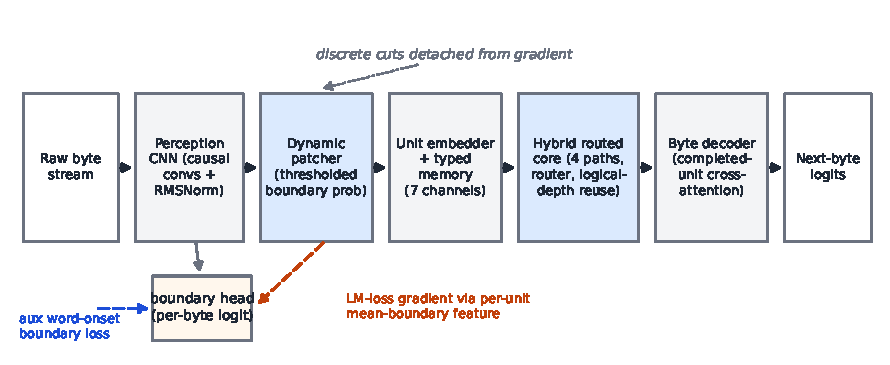
\includegraphics[width=\linewidth]{figures/fig1_pipeline.pdf}
  \caption{The end-to-end CFNA forward pass. The discrete segmentation is detached from the gradient; the boundary head is trained by the auxiliary word-onset loss and by the language-model loss through a per-unit mean-boundary feature.}
  \label{fig:pipeline}
\end{figure}

%%% ------------------------------------------------------------------
\section{Related Work and Contribution}
%%% ------------------------------------------------------------------

\subsection{Byte- and Character-Level Modeling}
ByT5~\cite{Xue2022} established that token-free byte models are viable and noise-robust at the cost of longer sequences. MegaByte~\cite{Yu2023} introduced the two-level patch/byte decomposition that CFNA's unit-core/byte-decoder split belongs to. The Byte Latent Transformer~\cite{Pagnoni2024} is closest in spirit with dynamic, entropy-driven patching; CFNA's patcher instead thresholds a single learned boundary probability trained jointly by word-onset self-supervision and the language-model gradient, with the discrete cuts detached. MambaByte~\cite{Wang2024} demonstrated byte modeling on a state-space backbone; CFNA uses a selective scan as one of four routed paths rather than the sole mixer. Unlike all of these, CFNA has not been evaluated on a standardized byte benchmark; its placement here is architectural, not results-based.

\subsection{State-Space and Hybrid Sequence Models}
Mamba~\cite{Gu2023} motivates the recurrent path, implemented by hand as an input-dependent selective scan. Jamba~\cite{Lieber2024} and Griffin~\cite{De2024} validate mixing recurrence with attention, but interleave block types by depth; CFNA computes all four mixers in every block and blends them per position with a learned router. Whether per-position fusion beats a plain interleave at equal compute is untested.

\subsection{Tokenizer-Based Frontier Designs}
The GPT-3~\cite{Brown2020}, PaLM~\cite{Chowdhery2022}, and LLaMA~\cite{Touvron2023} line is the backdrop for CFNA's departures; Chinchilla's compute-optimality lesson~\cite{Hoffmann2022} is encoded directly in the parameter-ladder presets (scale data with parameters; drop learning rate roughly with inverse width). The retrieval path draws on the RETRO lineage~\cite{Borgeaud2022}, kept at byte level so exact identifiers stay copyable. The typed memory descends conceptually from the protected cell state of long short-term memory~\cite{Hochreiter1997}. The calibration methodology for the authority classifier follows~\cite{Guo2017}.

\subsection{Contribution Statement}
\begin{enumerate}
\item A tokenizer-free two-level byte architecture whose unit segmentation is learned end to end (word-onset self-supervision plus a differentiable per-unit mean-boundary feature), with causality pinned by tests along every path.
\item A per-position four-path routed hybrid core (selective scan, local attention, sparse-global attention, retrieval cross-attention) with physical-block reuse over a configurable logical depth.
\item A native provenance/authority layer separating apparent authority from cryptographic authenticity, benchmarked against text-borne attack families rather than assumed.
\item A dual-backend implementation---mainstream framework and from-scratch NumPy autograd---required to reproduce a reference benchmark bit-identically across backends, operating systems, and Python versions.
\item A pre-registered acceptance-gate scaling methodology, and a complete empirical ledger including the negative results: an overfitting case study, a lost checkpoint, and a falsified architectural hypothesis.
\end{enumerate}

%%% ------------------------------------------------------------------
\section{Departures From the Established Process}
%%% ------------------------------------------------------------------

Table~\ref{tab:process} states, stage by stage, where CFNA's process departs from the established LLM production recipe. Every entry in the CFNA column is implemented and testable in the repository; none is aspirational. The table lists verified process differences, not superiority claims---the equal-compute comparison that could support a superiority claim has not been run.

\begin{table*}[!t]
\caption{The Established LLM Process vs.\ What CFNA Verifiably Does}
\label{tab:process}
\centering
\small
\begin{tabularx}{\textwidth}{lYY}
\toprule
\textbf{Stage} & \textbf{Established process} & \textbf{CFNA (verified in code)} \\
\midrule
Text ingestion & Subword tokenizer fit in advance; model inherits its vocabulary and failure modes & No tokenizer anywhere; raw bytes in and out; learned boundary head cuts variable-length units at run time \\
Sequence mixing & Homogeneous dense-attention stack, or fixed attention/state-space interleaves by depth & Four mixers computed in every block, blended per position by a learned router; physical blocks reused over logical depth \\
Trust and retrieval & Trust handled outside the model by prompt engineering or moderation & Typed data contract carries apparent authority and cryptographic authenticity into the prompt; Ed25519 gate benchmarked against attack families \\
Implementation & One implementation on one framework & Every layer built from primitives twice; bit-identical benchmark reproduction required across backends, OSs, Python versions \\
Scaling decisions & Scale first, evaluate after & Numeric acceptance gates written before each rung's runs; a rung cannot start until the previous gate clears \\
Reporting & Positive results published; failures rarely part of the record & Hypothesis ledger with a falsified central hypothesis; overfitting and checkpoint-loss incidents reported with numbers \\
\bottomrule
\end{tabularx}
\end{table*}

%%% ------------------------------------------------------------------
\section{Model Architecture}
\label{sec:arch}
%%% ------------------------------------------------------------------

\subsection{Perception and Dynamic Patching}
The perception encoder embeds each byte and applies a stack of causal one-dimensional convolutions---kernel-3, residual kernel-7, and residual dilated kernel-3 with dilation four---followed by root-mean-square normalization; causality is enforced by left padding. A small boundary head emits a per-byte boundary logit. At run time a boundary is cut when the learned boundary probability crosses a threshold and the current patch has reached a minimum length, or unconditionally at a maximum length. The head is trained two ways at once: an auxiliary loss against self-supervised word-onset targets (a boundary where a non-syntax byte follows a whitespace/punctuation byte), and the language-model gradient flowing through a per-unit mean-boundary feature that is projected and added to each unit's representation. The discrete cuts themselves are taken under no-gradient. The training objective is next-byte cross-entropy plus a weighted boundary cross-entropy; bits per byte is cross-entropy divided by $\ln 2$.

\subsection{Typed Multi-Timescale Memory}
Pooled per-unit features are projected to model width and passed through a typed gated recurrence whose read-out is added back onto the unit representations. Seven channels (semantic, structural, goal, evidence, uncertainty, authority, procedure) each keep a fixed retention timescale---uncertainty fastest at $0.90$, authority slowest at $0.999$---and an authority permission slot that throttles writes. Per step the cell computes forget, write, and read gates and a candidate update; the new cell state decays the old by retention times forget gate and adds the authority-masked, write-gated candidate. Section~\ref{sec:results} reports that the hoped-for per-channel specialization was \emph{falsified} at the scales tested.

\subsection{Routed Hybrid Core}
Every core block computes four outputs in parallel from the same normalized input: a selective state-space scan, local windowed attention, sparse-global attention keeping each query's top-$k$ causal keys, and retrieval cross-attention over retrieved byte context. A small router produces a per-position four-way softmax and blends the outputs; a gated feed-forward with residuals follows. Routing at each position depends only on that position's own causal path outputs. A few physical blocks are reused over a configurable \emph{logical depth}, decoupling computation depth from parameter count.

\begin{figure}[!t]
  \centering
  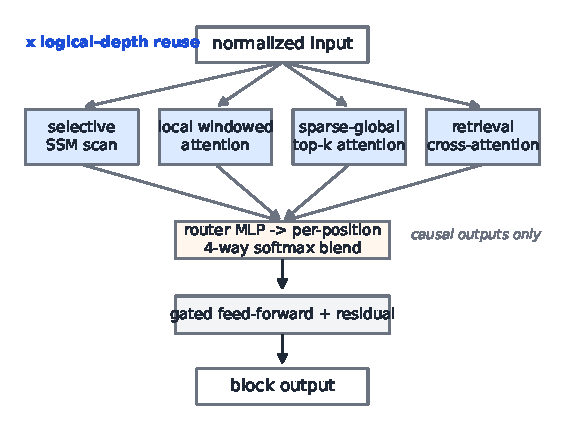
\includegraphics[width=\linewidth]{figures/fig2_coreblock.pdf}
  \caption{A single hybrid core block with per-position four-way routing.}
  \label{fig:coreblock}
\end{figure}

\subsection{Byte Decoder and Retrieval Encoding}
The decoder embeds bytes, attends locally over byte history, cross-attends to \emph{completed} units under a causal byte-to-unit mask (a byte may attend only to units strictly before its own segment), optionally cross-attends to retrieved context, and projects to 256-way logits. The completed-unit masking keeps the two-level model a valid left-to-right autoregressive model. Retrieval is engineered for exact copying: each retrieved position exposes its left context as the matching key and an embedding of the byte itself as the copyable value, making retrieval an induction-style copy that can reproduce exact identifiers.

\subsection{Parameter Ladder}
Four counted-by-construction presets instantiate the architecture: 11.1M (the only rung trained to date), 34.4M, 92.1M, and $\approx$337M. The largest constructs and forwards but has never been trained; its weights are random and only a scaling test verifies it builds at the stated size.

%%% ------------------------------------------------------------------
\section{Data and Training Procedure}
%%% ------------------------------------------------------------------

\subsection{Corpus Discipline}
A registry enumerates 22 licensed sources with page/file URLs, license labels, and intended training phase; two datasets are excluded for licensing reasons and the exclusions are annotated in the registry. For instruction tuning, a deterministic builder assembles a conversational dataset in the canonical prompt format: validate, deduplicate, cap any register at 25\% of the total, split and shard from a fixed seed, and verify zero train/validation/test leakage by hash. The committed manifest records 57{,}343 accepted records after deduplication and 54{,}685 after register caps (arithmetic and classification each held to 13{,}671---the remedy for a prior dataset that was 77\% arithmetic). The dataset regenerates bit-for-bit from the seed on any machine.

\subsection{Objectives and the Prompt-Format Contract}
Pretraining minimizes next-byte cross-entropy plus the boundary loss. Supervised fine-tuning masks the loss to assistant-response bytes only (including the end marker), enforced by a test asserting prompt bytes contribute zero gradient. One canonical prompt layout---system, user, evidence (each item carrying source id, authority, and authenticity), optional plan, assistant, end marker---is shared byte-for-byte by training and inference and stamped into every checkpoint; unstamped checkpoints resolve to the legacy format. This machinery exists because of a measured incident (Section~\ref{sec:results}).

\begin{table}[!t]
\caption{Validated Corpus of the 2026-07-02 Session (0.367~GB, 142 Shards)}
\label{tab:corpus}
\centering
\begin{tabular}{lr}
\toprule
Component & Size \\
\midrule
Permissively licensed code & 151.9~MB \\
Educational expository text & 120.0~MB \\
Books (incl.\ 21 owner-curated public-domain texts) & 54.8~MB \\
Training-loop traces & 40.0~MB \\
\bottomrule
\end{tabular}
\end{table}

%%% ------------------------------------------------------------------
\section{Engineering and System Implementation}
\label{sec:engineering}
%%% ------------------------------------------------------------------

\subsection{Dual Backends and Bit-Identical Reproduction}
The primary backend builds every layer from primitives on a mainstream framework used purely as an autograd/optimizer substrate, with mixed-precision hardening: normalization statistics in full precision under half-precision autocast, and dtype-aware masked softmax so fully-masked rows degrade to exact zeros. The second backend is a from-scratch reverse-mode autograd engine in NumPy at double precision (broadcasting-correct gradient accumulation; finite-difference checks). The same architecture, optimizer, evaluation harness, and authority classifier run on both. The payoff: a provenance benchmark reproduces \textbf{bit-identically} across operating systems (Windows/Linux), Python versions (3.13/3.11), and backends---strong evidence that results are properties of the specification, not of a numerical environment.

\subsection{Checkpointing as a Tested Contract}
Checkpoints are written atomically (write-then-rename); the best checkpoint is selected by validation, never by last step; resume restores shard, step, and optimizer moments. Two real incidents harden the story: a sandbox restart mid-run was caught cleanly by resume; and a best checkpoint at 1.313 held-out bits per byte was \emph{lost} to an unpersisted cloud runtime, after which a 30-minute auto-backup daemon was added. Both are reported because the reliability claim is only credible if it includes its failures. At the time of writing the test suite collects 249 tests, pinning causality along every path, the response-only mask, save/resume continuity, best-by-validation selection, stop-sequence termination, the prompt-format round trip, and mixed-precision numerics.

\begin{figure}[!t]
  \centering
  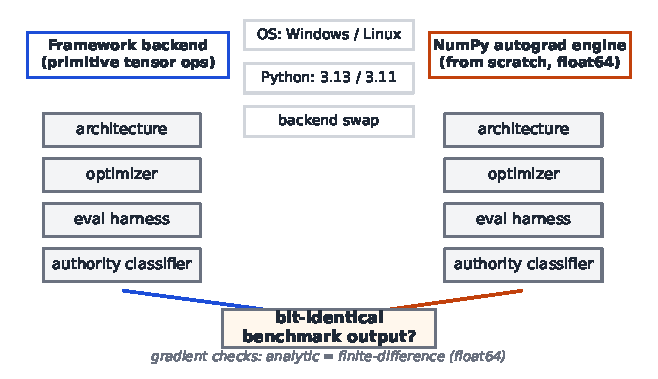
\includegraphics[width=\linewidth]{figures/fig3_dualbackend.pdf}
  \caption{The dual-backend equivalence harness.}
  \label{fig:dualbackend}
\end{figure}

%%% ------------------------------------------------------------------
\section{Results and Evaluation}
\label{sec:results}
%%% ------------------------------------------------------------------

\subsection{Base Pretraining}
Table~\ref{tab:session} summarizes the central positive result: the 2026-07-02 A100-40GB session. Table~\ref{tab:milestones} records the qualitative milestones observed along the loss curve, because they show what the loss buys. Continued training in a later session reached a best held-out 1.313 bits per byte ($\approx$168 additional minutes); coherent greedy prose first appeared near 1.31. That checkpoint no longer exists to re-evaluate (Section~\ref{sec:engineering}); the figure is reported as observed but unrecoverable. At session cutoff, training bits per byte ($\approx$1.2) still ran well below held-out (1.785) with the curve descending: at 0.367~GB, the 11M rung was data-limited, not capacity-limited.

\begin{table}[!t]
\caption{Base Pretraining Session (11.1M Parameters, From Scratch)}
\label{tab:session}
\centering
\begin{tabular}{lr}
\toprule
Metric & Value \\
\midrule
Held-out bits/byte, start $\to$ end & $4.515 \to 1.785$ \\
Steps / wall-clock & 7{,}524 / 55~min \\
Throughput & $\approx$37{,}000 byte-targets/s \\
Pre-registered SFT gate ($<1.8$) & cleared at min.\ 51 (1.797) \\
Sequence length / batch / precision & 256 / 64 / fp16 autocast \\
Later best (checkpoint lost) & 1.313 \\
\bottomrule
\end{tabular}
\end{table}

\begin{table}[!t]
\caption{Qualitative Milestones Along the Loss Curve (Greedy/Sampled Probes)}
\label{tab:milestones}
\centering
\small
\begin{tabularx}{\columnwidth}{lY}
\toprule
Held-out bpb & Observed behavior \\
\midrule
$\approx$2.67 & Greedy loops (``the the of the''); code prompt yields newline only \\
$\approx$2.11 & Morphologically legal invented words; English sentence rhythm \\
$\approx$2.03 & Indented Python with a recognizable assertion call; prose registers separate \\
$\approx$1.31 & First coherent greedy sentence (observed; checkpoint unrecoverable) \\
\bottomrule
\end{tabularx}
\end{table}

\subsection{Supervised Fine-Tuning: An Overfitting Case Study}
A maximum length of 384 bytes combined with a $\approx$300-byte system prompt filtered $\approx$20{,}000 dialogue pairs to 429 examples (8 validation). Validation loss bottomed at 1.246 at step 225, then rose to $\approx$1.94 by step 2{,}425 while training loss fell to $\approx$0.05---textbook memorization; the trainer of that era kept only final weights, so the deployed checkpoint was the overfit endpoint. A chat probe still produced the project's first turn-taking behavior (a greeting answered with a garbled greeting). Fixes landed the same session: maximum length 1{,}024, best-by-validation atomic saves, early stopping. The episode replicates the project's most-repeated lesson: fine-tuning \emph{shapes} competence but cannot \emph{create} it.

\subsection{Structure Generalizes Before Content}
An earlier NumPy-engine study fine-tuned a 112{,}709-parameter model on 100{,}000 synthetic conversations (5{,}000/5{,}000 held out, zero leakage). Held-out byte accuracy reached 89.06\%, but arithmetic was memorized as \emph{shape}, not procedure: strict check-pass 2.1\% on novel operand pairs and 4.7\% even on exact training pairs. A naive metric showed 83\% apparent parity accuracy that collapsed to 1/24 under a stricter check---a metric-design failure reported against the project itself. Consequence: choice-ranking metrics are required alongside generative ones, and checkpoints may not be discarded on generative exact-match alone.

\subsection{The Prompt-Format Drift Incident}
A checkpoint predating the canonical format scored 0.906 teacher-forced byte accuracy in its native format and 0.524 under the mismatched canonical format---a silent 38-point regression that looked like a weak model but was purely an evaluation-format mismatch. This motivated format stamping in every checkpoint and a tested rule: never compare accuracies across formats and call the difference model quality.

\subsection{The Provenance/Authority Result}
The strongest defensible result is in the symbolic layer. A from-scratch, calibrated authority classifier (expected calibration error 0.004~\cite{Guo2017}) holds \textbf{zero acceptance of poisoned documents} across text-borne attack families---impersonation, laundering, citation spoofing, paraphrase, Unicode confusables---on a blind set from an independent code path, while naive baselines poison at 0.75--1.00. A feature-identical ``perfect spoof'' residual (0.278 acceptance) was proven an information-theoretic ceiling and closed by the Ed25519 gate, driving poison acceptance to zero with calibrated abstention. Removing the labels-given assumption costs measured accuracy: oracle 1.000 drops to a predicted 0.838 end to end. Table~\ref{tab:provenance} reports the integrated ablations. This benchmark is the artifact that reproduces bit-identically across environments.

\begin{table}[!t]
\caption{Integrated Provenance Pipeline and Ablations}
\label{tab:provenance}
\centering
\begin{tabular}{lrr}
\toprule
Configuration & Answer acc. & Poison acc. \\
\midrule
Full pipeline & 0.920 & 0.000 \\
$-$ retrieval & 0.480 & --- \\
$-$ provenance gate & --- & 0.260 \\
$-$ verifier (unsupported-claim rate) & \multicolumn{2}{r}{$0.000 \to 0.090$} \\
\bottomrule
\end{tabular}
\end{table}

\subsection{A Falsified Hypothesis}
The differentiation story leaned on typed memory channels specializing into distinct roles. A probe trained a small model on tasks with distinct memory demands, then zeroed channels: removing \emph{all} typed channels raised loss only on long-range recall ($\approx$3.5\%) and near-zero elsewhere; removing any \emph{single} channel changed loss by $<$0.3\% on every task. The channels behave as a redundant pool. The specialization hypothesis is recorded as \textbf{falsified} at this scale and training, and the differentiation argument no longer rests on it.

\begin{figure}[!t]
  \centering
  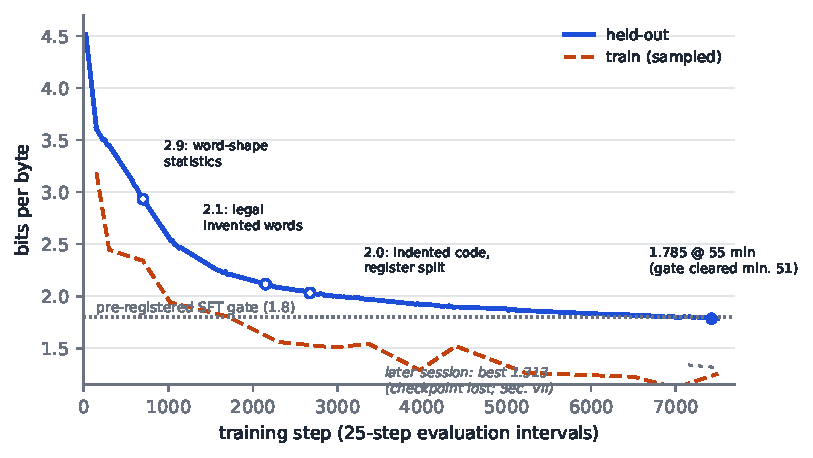
\includegraphics[width=\linewidth]{figures/fig4_curve.pdf}
  \caption{The base pretraining curve with pre-registered gate and milestones.}
  \label{fig:curve}
\end{figure}

%%% ------------------------------------------------------------------
\section{Claim Classification}
%%% ------------------------------------------------------------------

\begin{table*}[!t]
\caption{Claim Type and Status}
\label{tab:claims}
\centering
\small
\begin{tabularx}{\textwidth}{lYY}
\toprule
\textbf{Claim} & \textbf{Type} & \textbf{Status} \\
\midrule
Architecture trains from scratch to fluent-shaped output & Empirical (logged run) & Verified; 4.515$\to$1.785 bpb in 55 min, gate cleared in-session \\
Later best 1.313 bpb; coherent greedy prose near 1.31 & Empirical (logged, unrecoverable) & Observed; checkpoint lost; re-verification requires retraining \\
Fine-tuning shapes but cannot create competence & Empirical, replicated at two scales & Supported (61-example, 429-example, and gate-conditioned outcomes) \\
Zero poison acceptance across text-borne attack families & Empirical (blind benchmark) & Verified; reproduces bit-identically across environments \\
Typed-channel specialization & Hypothesis & \textbf{Falsified} at tested scale \\
Per-position routing beats depth interleaving & Hypothesis & Untested (needs equal-compute baseline) \\
Externally comparable loss numbers & --- & Not available; validation set is project-private \\
Superiority over conventional transformers & --- & Not claimed; experiment not run \\
\bottomrule
\end{tabularx}
\end{table*}

%%% ------------------------------------------------------------------
\section{Scope and Limitations}
%%% ------------------------------------------------------------------

\begin{table}[!t]
\caption{Limitations and Future Requirements}
\label{tab:limits}
\centering
\scriptsize
\begin{tabularx}{\columnwidth}{p{0.30\columnwidth}YY}
\toprule
\textbf{Limitation} & \textbf{Current status} & \textbf{Requirement} \\
\midrule
Trained scale & 11.1M only & Train 35M/90M rungs through gates \\
Private validation set & Not externally comparable & enwik8/text8 evaluation \\
No baseline face-off & Works, not ``wins'' & Equal-compute transformer baseline \\
Neural/symbolic split & Two islands, data contract only & Condition generation on authority \\
Typed memory & Specialization falsified & Re-engineer, re-probe \\
One simulated gate & A tie true by construction & Real pipeline in the loop \\
\bottomrule
\end{tabularx}
\end{table}

This paper is small-scale and classical. The 1.785 and 1.313 bits-per-byte figures are on the project's own held-out split and cannot be compared to published numbers. No equal-compute, equal-data transformer has been trained alongside CFNA, so no claim is made that the architecture beats a conventional design at matched budget. The learned byte core and the symbolic provenance layer are connected only by a data contract: the neural model does not yet condition on authority signals, so the strongest provenance result is a property of the symbolic layer, not of an integrated model. One provenance evaluation contained a full-system/contract-only tie that was guaranteed by construction because the pipeline was simulated; it is flagged rather than counted.

%%% ------------------------------------------------------------------
\section{Assumptions and Future Work}
%%% ------------------------------------------------------------------

\textbf{Assumptions.} (1)~Held-out bits per byte on the project corpus is a meaningful quality proxy, though not externally comparable. (2)~The 1.8 gate is a project convention, not a derived threshold. (3)~Synthetic conversational data is a fair small-scale proxy for instruction behavior. (4)~The provenance attack families represent realistic text-borne attacks; key compromise is out of scope and handled by revocation. (5)~Counted parameter labels track effective capacity in the usual way.

\textbf{Future work.} (1)~Train the 35M rung to its pre-registered gates (bpb $\le 1.5$; choice-ranking $\ge$15 points over chance on $\ge$3 subjects; $\ge$60\% valid stop-terminated answers; 5/5 grammatical transcripts), then 90M, and only then consider 337M. (2)~Run enwik8/text8 so loss numbers become externally comparable. (3)~Run the equal-compute plain-transformer baseline. (4)~Integrate the neural core with the provenance layer so generation conditions on authority-gated evidence. (5)~Re-engineer typed-channel specialization with per-channel read-outs or channel-specific losses and re-probe. (6)~Replace the simulated provenance evaluation with the learned pipeline in the loop and add an externally authored blind benchmark. (7)~Retrain past the lost 1.313 checkpoint under the new auto-backup regime and confirm coherent-prose emergence reproducibly. (8)~Complete the deferred verifier-guided fine-tuning stages once a base model worth revising exists.

%%% ------------------------------------------------------------------
\section{Conclusion}
%%% ------------------------------------------------------------------

CFNA demonstrates that a tokenizer-free, from-scratch, provenance-gated language model can be built, trained, and audited end to end by a single-owner research effort: an 11.1M-parameter model reached fluent-shaped output from raw bytes in under an hour of A100 time under a pre-registered gate; a cryptographic provenance layer holds zero poison acceptance on blind text-borne attacks; and the entire system reproduces a reference benchmark bit-identically across two independent implementations. The honest position is equally clear: the model is small, its loss numbers are not yet externally comparable, its architectural advantages over a conventional transformer are untested at matched budget, and one of its central architectural hypotheses is falsified. What distinguishes this work is therefore the verified \emph{process}---no borrowed machinery, trust inside the data contract, gates before scaling, and failures published beside successes---and the complete, reproducible ledger that lets every claim in this paper be checked against a file, a test, or a logged run.

\section*{Acknowledgment}
The author thanks the automated review passes that audited every claim in this manuscript against the repository's code and committed experiment reports, and that removed one inaccurate mechanism description before publication.

\begin{thebibliography}{19}

\bibitem{Brown2020}
T.~B. Brown \emph{et al.},
``Language models are few-shot learners,''
in \emph{Advances in Neural Information Processing Systems}, 2020.

\bibitem{Vaswani2017}
A.~Vaswani \emph{et al.},
``Attention is all you need,''
in \emph{Advances in Neural Information Processing Systems}, 2017.

\bibitem{Gu2023}
A.~Gu and T.~Dao,
``Mamba: Linear-time sequence modeling with selective state spaces,''
arXiv preprint arXiv:2312.00752, 2023.

\bibitem{Xue2022}
L.~Xue \emph{et al.},
``ByT5: Towards a token-free future with pre-trained byte-to-byte models,''
\emph{Trans.\ Assoc.\ Comput.\ Linguistics}, vol.~10, pp.~291--306, 2022.

\bibitem{Yu2023}
L.~Yu \emph{et al.},
``MEGABYTE: Predicting million-byte sequences with multiscale transformers,''
in \emph{Advances in Neural Information Processing Systems}, 2023.

\bibitem{Pagnoni2024}
A.~Pagnoni \emph{et al.},
``Byte latent transformer: Patches scale better than tokens,''
arXiv preprint arXiv:2412.09871, 2024.

\bibitem{Wang2024}
J.~Wang, T.~Gangavarapu, J.~N. Yan, and A.~M. Rush,
``MambaByte: Token-free selective state space model,''
arXiv preprint arXiv:2401.13660, 2024.

\bibitem{Lieber2024}
O.~Lieber \emph{et al.},
``Jamba: A hybrid transformer--Mamba language model,''
arXiv preprint arXiv:2403.19887, 2024.

\bibitem{De2024}
S.~De \emph{et al.},
``Griffin: Mixing gated linear recurrences with local attention for efficient language models,''
arXiv preprint arXiv:2402.19427, 2024.

\bibitem{Hoffmann2022}
J.~Hoffmann \emph{et al.},
``Training compute-optimal large language models,''
arXiv preprint arXiv:2203.15556, 2022.

\bibitem{Chowdhery2022}
A.~Chowdhery \emph{et al.},
``PaLM: Scaling language modeling with Pathways,''
arXiv preprint arXiv:2204.02311, 2022.

\bibitem{Borgeaud2022}
S.~Borgeaud \emph{et al.},
``Improving language models by retrieving from trillions of tokens,''
in \emph{Proc.\ Int.\ Conf.\ Machine Learning}, 2022.

\bibitem{Hochreiter1997}
S.~Hochreiter and J.~Schmidhuber,
``Long short-term memory,''
\emph{Neural Computation}, vol.~9, no.~8, pp.~1735--1780, 1997.

\bibitem{Zhang2019}
B.~Zhang and R.~Sennrich,
``Root mean square layer normalization,''
in \emph{Advances in Neural Information Processing Systems}, 2019.

\bibitem{Shazeer2020}
N.~Shazeer,
``GLU variants improve transformer,''
arXiv preprint arXiv:2002.05202, 2020.

\bibitem{Touvron2023}
H.~Touvron \emph{et al.},
``LLaMA: Open and efficient foundation language models,''
arXiv preprint arXiv:2302.13971, 2023.

\bibitem{Bernstein2012}
D.~J. Bernstein, N.~Duif, T.~Lange, P.~Schwabe, and B.-Y. Yang,
``High-speed high-security signatures,''
\emph{J.\ Cryptographic Engineering}, vol.~2, pp.~77--89, 2012.

\bibitem{Guo2017}
C.~Guo, G.~Pleiss, Y.~Sun, and K.~Q. Weinberger,
``On calibration of modern neural networks,''
in \emph{Proc.\ Int.\ Conf.\ Machine Learning}, 2017.

\end{thebibliography}

\IfFileExists{author_photo.jpg}{%
\begin{IEEEbiography}[{\includegraphics[width=1in,height=1.25in,clip]{author_photo.jpg}}]{Luis M. Minier}
is an independent researcher based in New York, NY, USA. He is the creator of CFNA and the nueronce research system. His research interests include byte-level language models, learned segmentation, hybrid state-space architectures, cryptographic provenance for machine learning, and reproducible small-scale foundation-model research.
\end{IEEEbiography}
}{%
\section*{Biography}
\begingroup\footnotesize
\noindent\textbf{Luis M. Minier} is an independent researcher based in New York, NY, USA. He is the creator of CFNA and the nueronce research system. His research interests include byte-level language models, learned segmentation, hybrid state-space architectures, cryptographic provenance for machine learning, and reproducible small-scale foundation-model research.\par
\endgroup
}

\end{document}
